\documentclass[tekniskrapport/tech.tex]{subfiles}

\begin{document}

\section{Kommunikationsmodul}
Kommunikationsmodulen styr bilen och kommunicerar med fjärrklienten.
Sensorvärden från sensormodulen tolkas av kommunikationsmodulen som därefter
skickar felvärden till styrmodulen.

Bildbehandling utförs av kommunikationsmodulen för att
avgöra bilens position i vägfilen och upptäcka stopplinjer. Med hjälp av
kamerans bilder på vägen skapas ett felvärde som kan användas för att justera
taxins riktning.

Kommunikation med fjärrklienten sköts av kommunikationsmodulen för
att skicka sensorvärden och annan relevant information. Modulen tar
även emot uppdrag.

Autonomitet utförs av kommunikationsmodulen för att utföra uppdraget.
Kommunikationsmodulen hämtar sensordata från sensormodulen och bildbehandlar
kamerabilderna för att utföra beslut i realtid. Besluten skickas i form av fel-
och styrvärden till styrmodulen.

Kommunikationsmodulens program är skriven i både C och C++. Bildbehandlingen är
skriven i C++ medan resten av programmet är implementerad med C. De olika
delarna kompileras separat och länkas sedan ihop med kompilatorn för C++.
Programmet består av tre trådar; en huvudtråd som hanterar uppdrag och
bildbehandlar, samt en tråd som sköter kommunikation via SPI och en som svarar
på kommandon från fjärrklienten via TCP/IP. SPI:n och servern sköts i separata
trådar eftersom de väntar mycket och blockerar den nuvarande tråden.


\subsection{Hårdvaruimplementation} 
% TODO

\paragraph{Programstruktur}
Programmet på kommandomodulen består av följande filer

\begin{labeling}{wwww}
    \item[server.c] Server som anropar kommandofunktioner vid förfrågan från
        klient från separat tråd.
	\item[spi.c] Lågnivåfunktioner för SPI.
    \item[bus.c] Hantering av SPI-buss, utför kommandon på bussen och anropar
        signalhanterare från separat tråd.
    \item[ip/img\_proc.cpp] Bildbehandling med OpenCV.
    \item[objective.c] Utförarande av uppdrag.
    \item[main.c] Huvudloop och implementation av signalhanterare för buss och
        server.
\end{labeling}

\paragraph{Huvudtråden} startar servern och busshanteraren. Därefter startar
den huvudloopen som antingen tar styrvärden utifrån användarens kommandon via
servern eller från uppdragshanteraren med hjälp av bildbehandling. Därefter schemaläggs
skrivning av de nya styrvärdena till styrmodulen. Dessutom schemaläggs hämtning
av sensorvärden från sensorerna.

\paragraph{Server}
% TODO

\paragraph{Busshanterare} 
% TODO

\subsection{Bildbehandling}
% TODO
Bildbehandlings processen sker genom ett program skrivet i C++.
\paragraph{Upptäkt av linjer}
Upptäckandet av linjer/kanter på banan sker genom hanteringen av varje bild/frame som programmet tar emot från kameran. Varje bild går igenom en process som börjar med att förberedda bilden genom att filtrera den för att först underlätta kanters upptäckande och sedan linjerna inom ett bestämt område av intresse (Region of Interest ROI).

Processen börjar med att filtrera bilden med den så kallade Gauss filter där bilden faltas med en Gauss kernel med tanke på att filtrera bort brus. Den filtrerade bilden omvandlas sedan till en monokromatisk bild vilket underlättar bildbehandlingen och som är möjligt tack vare att bildbehandlingsprogrammet inte använder sig utav specifika färger för att upptäcka linjer på vägen utan det arbetar med de linjerna inom ROI och klassar dem enligt deras lutning och position. Det här innebär att upptäckandet av linjer ska vara möjligt utfört oberoende på vilka färger vägen kunde ha. 

Det sista steget innan kanterna upptäcks är att segmentera bilden genom att från openCV använda threshold funktionen som erbjuder olika typer av threshold operationer vilka möjliggör att skilja mellan olika region/objekt som önskas analysera baserad på hur intensiteten hos varje pixel varierar mellan objektet och bakgrunden. Programmet använder sig av Otsu threshold metod vilken själv räknar ut en threshold värdet som bäst passar bilden. Den använda threshold funktionen returnera den nya bilden vilken visas på bilden...

Nu när bilden är förbered för kanters upptäckande används funktionen Canny (från openCv), som applicerar Canny algoritmen vilken identifierar alla kanter som finns i bilden. Resultatet visas på bilden ... 

Som tidigare nämnts, upptäcks linjerna inom ROI. ROI bestäms baserad på hur mycket av bilden vill användas för att hitta linjer; hur mycket som är tillräckligt för tolkningen och senare hanteringen av alla linjer som hittas på vägen. ROI är en polygon av 6 punkter som enkelt kan anpassas vid behov och som visas på bilden ...   

Efter att bilden är hel filtrerad och ROI bestämd, används Hough transformen för att hitta linjer enligt bestämda parametrar som varje linje ska uppfylla i transformen för att bli klassa som linje. OpenCV erbjuder två typer av funktioner som applicerar transformen och programmet använder sig av den probabilistiska metoden vilken ökar beräknings hastighet utan att minska precisionen. Efter användningen av Hough transformen kan programmet tolka de upptäckade linjerna.

  
\paragraph{Tolkning av linjer}

\subsection{Uppdrag}

\begin{wrapfigure}{r}{0.3\linewidth}
    \begin{center}
        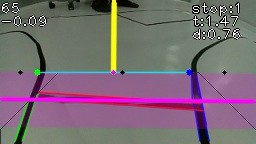
\includegraphics[width=\linewidth]{tekniskrapport/figures/opencv.jpg}
    \end{center}
    \caption{Klassificering och tolkning av linjer från kamera.}
\end{wrapfigure}

\subsubsection{Uppdrag} \label{sec:comm-mission}
% TODO
För att utföra uppdraget kommer en kö av kommandon tas emot från fjärrklienten.
När uppdraget börjar kör taxin framåt och följer filen med hjälp av
bildbehandling och reglering. Inför varje stopplinje tas ett kommando från kön
och utförs. Om ett hinder upptäcks under uppdraget kommer bilen att stanna
tills hindret har försvunnit eller eventuellt passera hindret. När ett visst
antal stopplinjer har passerats och kön är tom är uppdraget avklarat. Nedan är
en lista av alla möjliga kommandon hur de utförs.
\begin{labeling}{wwww}
    \item[\commIgnore] Kör förbi stopplinjen utan att stanna.
    \item[\commStop] Stanna framför stopplinjen, fortsätt efter några sekunder
    om kön inte är tom.
    \item[\commPark] Parkera i fickan till höger efter stopplinjen, lämna
    parkeringen och fortsätt efter några sekunder om kön inte är tom.
    \item[\commEnter] Sväng höger in i rondellen och hitta rondellens körfil.
    \item[\commContinue] Kör förbi stopplinje och håll till vänster.
    \item[\commExit] Sväng höger ut ur rondellen och hitta körfilen.
\end{labeling}

\end{document}
